\documentclass[12pt,a4paper,openany]{report}
%%%% JNLP 
\usepackage{lmodern}
\usepackage{xcolor}
\usepackage[utf8]{inputenc}
\usepackage[T1]{fontenc}
\usepackage[francais]{babel}
\usepackage[top=1.7cm, bottom=1.7cm, left=1.5cm, right=1.5cm]{geometry}
\usepackage{pdfpages}
\usepackage{listingsutf8}
\usepackage{fancyhdr}
\usepackage{multido}
\usepackage{amssymb}
\usepackage{tikz}
\usepackage{ifthen}
\usepackage{makeidx}
\usepackage[urlbordercolor={1 1 1}, linkbordercolor={1 1 1}, urlcolor=blue]{hyperref}
\usepackage{wrapfig}
\usepackage{longtable}
\usepackage{array}
\usepackage{float}

%\newCommand{\footGauche}{} Université paul sabatier Toulouse III
\newcommand{\footCentre}{}
%\newCommand{\footDroite}{} Numéro de page
\newcommand{\premierDestinataire}{Monsieur Max \bsc{Chevalier}}
\newcommand{\rolePremierDestinataire}{Responsable projets}

\newcommand{\secondDestinaire}{Monsieur Thierry \bsc{Millan}}
\newcommand{\roleSecondDestinaire}{Client}

\newcommand{\troisiemeDestinaire}{Madame Caroline \bsc{Kross}}
\newcommand{\roleTroisiemeDestinaire}{Tutrice}

\newcommand{\quatriemeDestinaire}{}
\newcommand{\roleQuatriemeDestinaire}{}

\newcommand{\cinquiemeDestinaire}{}
\newcommand{\roleCinquiereDestinaire}{}
\newcommand{\titreDocument}{Analyse et conception}
\newcommand{\separateur}{\begin{center}\rule{12.6cm}{.5pt}\end{center}}
	


\date{\today}

\chead{\headCentre}
\rhead{\headDroite}
\lhead{\headGauche}
\makeindex
\lfoot{Université Paul Sabatier Toulouse III}
\rfoot{--~\thepage~--}
\cfoot{\footCentre}
\makeglossary
\makeatletter
\def\clap#1{\hbox to 0pt{\hss #1\hss}}%
\def\ligne#1{%
\hbox to \hsize{%
\vbox{\centering #1}}}%
\def\haut#1#2#3{%
\hbox to \hsize{%
\rlap{\vtop{\raggedright #1}}%
\hss
\clap{\vtop{\centering #2}}%
\hss
\llap{\vtop{\raggedleft #3}}}}%
\def\bas#1#2#3{%
\hbox to \hsize{%
\rlap{\vbox{\raggedright #1}}%
\hss \clap{\vbox{\centering #2}}%
\hss
\llap{\vbox{\raggedleft #3}}}}%
\def\maketitle{%
\thispagestyle{empty}\vbox to \vsize{%
\haut{}{\@blurb}{}
\begin{flushleft}
	\vspace{1cm}
	Antoine de \bsc{Roquemaurel}\\ 
	Mathieu \bsc{Soum}\\
	Geoffroy \bsc{Subias}\\
	Marie-Ly \bsc{Tang}\\
	\textit{Groupe B}\\
\end{flushleft}
\begin{flushright}
	\vspace{-3cm}
	\ifthenelse{\equal{\premierDestinataire}{}}{
	}
	{
		Pour \premierDestinataire(\rolePremierDestinataire)\\
	}
	\ifthenelse{\equal{\secondDestinaire}{}}{
	}
	{
		Pour \secondDestinaire(\roleSecondDestinaire)\\
	}
	\ifthenelse{\equal{\troisiemeDestinaire}{}}{
	}
	{
		Pour \troisiemeDestinaire(\roleTroisiemeDestinaire)\\
	}
	\ifthenelse{\equal{\quatriemeDestinaire}{}}{
	}
	{
		Pour \quatriemeDestinaire(\roleQuatriemeDestinaire)\\
	}
	\ifthenelse{\equal{\cinquiemeDestinaire}{}}{
	}
	{
		Pour \cinquiemeDestinaire(\roleCinquiereDestinaire)\\
	}
\end{flushright}
\vfill
\vspace{1cm}
\begin{flushleft}
\usefont{OT1}{ptm}{m}{n}
\huge \@title
\end{flushleft}
\par
\hrule height 4pt
\par
\begin{flushright}
\usefont{OT1}{phv}{m}{n}
\Large \@author
\par
\end{flushright}
\vspace{1cm}
\vfill
\vfill
\bas{}{\@location, le \@date}{}
}%
\cleardoublepage
}
\def\date#1{\def\@date{#1}}
\def\author#1{\def\@author{#1}}
\def\title#1{\def\@title{#1}}
\def\location#1{\def\@location{#1}}
\def\blurb#1{\def\@blurb{#1}}
\date{\today}
\author{}
\title{}
\location{Amiens}\blurb{}
\makeatother
\title{\titreDocument}
\author{Bibliothèque d'objets graphiques UML}

\location{Toulouse}
\blurb{%
Université Paul Sabatier -- Toulouse III\\
IUT A - Toulouse Rangueil\\
\textbf{Projet tuteuré}\\[1em]
}%



\pagestyle{fancy}

\begin{document}
%\setcounter{tocdepth}{4}
	\maketitle
	\newpage
	\tableofcontents
	\chapter*{Avant-propos}
\nouveauChapitre
\addcontentsline{toc}{chapter}{Avant-propos}
\section*{Présentation du projet}
\addcontentsline{toc}{section}{Présentation du projet}
	LibUML est une 
	\glo{bibliothèque}{Bibliothèque}{Composant programmé dans un langage donné fournissant des méthodes permettant d'effectuer des tâches voulut} 
	d'objets graphiques représentant les différents éléments de modélisation de la norme 
	\glo{UML}{UML}{(Unified Modeling Language) Langage de modélisation graphique à base de pictogramme.  Il est apparu dans le monde du génie logiciel dans le cadre de la conception orientée objet. Ce langage est composé de différents diagrammes, allant du développement à la simple analyse des besoins.} 
	2\footnote{Unified Modelling Language}.
	Celle-ci à été développé dans le cadre des projets tuteurés à l'IUT\footnote{Institut Universitaire de Technologies} 'A' de Toulouse. 
	Nous l'avons développée en \glo{Java}{Java}{Langage de programmation orienté objet moderne, il compile le programme pour ensuite l'exécuter sur une machine Java, ainsi le programme une fois compilé peut être exécuté sur différentes plateformes (Windows, Linux, Mac OS X, \ldots).} 
	et conçut comme une bibliothèque pouvant être utilisée dans des programmes Java comme composant. 
	Vous pouvez vous en servir pour développer un outil complet de modélisation UML par exemple.
	\paragraph{}	
	Cette bibliothèque permet de faire différentes choses dans le cadre de la conception UML, une fois la
	que vous aurez compris le fonctionnement de libUML vous pourrez:
	\begin{itemize}
		\item Créer des éléments de modélisation 
			\begin{itemize}
				\item Acteur actif ou passif
				\item Traitement
				\item Cas d'utilisation
				\item Classe
			\end{itemize}
		\item Relier ses composants via différents types de flèches
			\begin{itemize}
				\item Agrégation
				\item Composition
				\item Association binavigable ou mononavigable
				\item Messages synchrones ou asynchrones
				\item Généralisation
			\end{itemize}
		\item Supprimer des éléments et flèches
		\item Modifier le contenu des éléments et flèches
		\item Redimensionner les éléments de modélisation
	\end{itemize}
	\paragraph{}
Ce document à pour but de vous présenter le fonctionnement de la bibliothèque UML et de son démonstrateur. 

\section*{Présentation du groupe}
\addcontentsline{toc}{section}{Présentation du groupe}
	Notre groupe projet est composé de quatre étudiants de deuxième année de DUT Informatique à l'IUT 'A' de Toulouse, voici la composition de l'équipe: 
	\begin{itemize}
		\item Antoine de \bsc{Roquemaurel} 
		\item Mathieu \bsc{Soum} 
		\item Geoffroy \bsc{Subias}
		\item Marie-Ly \bsc{Tang} 
	\end{itemize}
	\section*{Téléchargements}
\addcontentsline{toc}{section}{Téléchargements}
	Nous vous avons envoyé deux archives zip par email, une contenant le projet Netbeans de la bibliothèque et du démonstrateur et une contenant la bibliothèque.
	\subsubsection*{Bibliothèque et démonstrateur}
	La première archive est donc un projet netbeans, cette archive contient notre bibliothèque et ses tests associés, le démonstrauteur mais
	également la bibliothèque \texttt{JGraphx} qui est indispensable au bon fonctionnement de notre bibliothèque. Nous ne garantissons le bon fonctionnement 
	de la bibliothèque qu'avec la version de \texttt{JGraphx} 1.8, celle-ci n'ayant pas été testé avec des versions différentes.

	Le projet netbeans de notre bibliothèque est également disponible en ligne, si vous souhaitez la télécharger de nouveau, elle est donc disponible à l'adresse suivante: \\
	$\rhd$ \url{http://telechargements.joohoo.fr/libUML/libUML-netbeans.zip}\\
	$\rhd$ \url{http://telechargements.joohoo.fr/libUML/JGraphX-1.8.jar}\\
	
	\subsubsection*{Documentation}
	Toute la documentation du projet est sous format \bsc{HTML}\footnote{HyperText Markup Language}, celle-ci ayant été générée grâce à Javadoc.

	Si dans ce manuel nous parlons d'une méthode et que vous n'en comprenez pas l'intéret, vous pouvez aller la chercher dans la documentation, pour chaque classe,
	le fonctionnement global de la classe est expliquée, l'utilité de chaque attribut, de chaque méthode, et ce que vous devez mettre dans les différents paramètres 
	des méthodes.  
	\paragraph{}
	Nous vous avons remis un .zip par email contenant quatre dossiers de documentation:
	\begin{itemize}
		\item La documentation privée de la \textit{bibliothèque} (Toutes les méthodes et tous les attributs)
		\item La documentation publique de la \textit{bibliothèque} (Seuls les méthodes et attributs publiques ou protégées)
		\item La documentation privée du \textit{démonstrateur} (toutes les méthodes du démonstrateur) 
		\item La documentation des \textit{tests unitaires} (Toutes les méthodes de tests)
	\end{itemize}
	\paragraph{}
	Celle ci est également disponible en ligne aux adresses suivantes: \\
	$\rhd$ \url{http://documentation.joohoo.fr/libUML/bibliothequePrivee/index.html}\\
	$\rhd$ \url{http://documentation.joohoo.fr/libUML/bibliothequePublique/index.html}\\
	$\rhd$ \url{http://documentation.joohoo.fr/libUML/demonstrateurPrivee/index.html}\\\label{docDemonstrateur}
	$\rhd$ \url{http://documentation.joohoo.fr/libUML/testsUnitaires/index.html}\\
	\paragraph{}
	Vous pouvez également accéder à la documentation de \texttt{JGraphX}, cela peut vous être utile dans certains cas.\\
	$\rhd$ \url{http://documentation.joohoo.fr/JGraphX/index.html}\\ 


	\newpage
\section*{Fonctionnement du document}
\addcontentsline{toc}{section}{Fonctionnement du document}
Ce document est un document expliquant notre approche pour développer une bibliothèque d'objets graphiques UML.\\

Dans ce dossier, vous pourrez repérer diverses notations, cette partie a pour but de vous expliquer les notations afin
que vous puissiez lire en toute sérénité.
\subsubsection*{Le glossaire}
Un mot dans le glossaire a une police particulière, vous pourrez savoir qu'un mot est dans le glossaire lorsque vous repérerez un mot avec la police suivante: 
\policeGlossaire{leMotDansLeGlossiare}. Si vous voyez cette police, vous pouvez donc vous référez à l'annexe \ref{glossaire} page \pageref{glossaire}.
\subsubsection*{Les noms de méthode, d'attribut ou de classe}
Les mots se référant à un nom présent dans du code ont une police particulière, une police type ``machine à écrire'', si vous voyez la police suivante, c'est que c'est un nom 
de méthode, d'attribut ou de classe: \texttt{uneFonction}.
\subsubsection*{Les noms de paquetage}
Les noms de paquetage utiliseront une police particulière, afin que l'on puisse les différencier d'une classe ou d'une méthode, vous les trouverez 
comme suit : \policePackage{unPaquetage}.
\subsubsection*{Les notes de bas de page}
Nous utilisons régulièrement des notes de bas de pages, pour donner un acronyme, pour expliquer plus en détail une notion, ces notes de bas de pages sont un numéro
en exposant, vous trouverez la note correspondante en bas de la page courante, comme ceci\footnote{Ceci est une note de bas de page}.
\subsubsection*{Les liens hypertextes}
Dans le document, nous pouvons faire référence à un lien d'un site web, tous les liens seront donc symbolisés par une petite puce, et une police particulière comme ceci:\\
	$\rhd$ \url{http://monLien.fr/index.html}\\
	Une liste de tous les liens présents dans le document est accessible en annexe \ref{listeLiens} page \pageref{listeLiens}.


	\newpage
	\chapter{Spécification des besoins}
	\section{Objectifs, champ d'application, limites du système}
	La demande de ce système émane de Monsieur Thierry \bsc{Millan}, enseignant à l'IUT\footnote{Institut Universitaire de Technologie}
	'A' Toulouse et chercheur à l'IRIT\footnote{Institut de Recherche Informatique de Toulouse},
	qui nous a demandé la création d'une bibliothèque d'objets graphiques représentant
	les différents éléments de modélisation de la norme \glo{UML}{UML}{(Unified Modeling Language) Langage de modélisation
	graphique à base de pictogramme. Il est apparu dans le monde du génie logiciel dans le cadre de la conception orientée
	objet. Ce langage est composé de différents diagrammes, allant du développement à la simple analyse des besoins.}
	\footnote{Unified Modeling Language} 2.0 en suivant un modèle de développement \glo{incrémental}
	{Incrément}{Fonctionnalité du logiciel, ayant un cycle de developpement lui étant propre (Analyse, Développement, Tests).
	Cette fonctionnalité doit être opérationnelle pour que l'incrément soit terminé. Il doit améliorer le logiciel
	par rapport à l'incrément précédent, et ne doit pas altérer les fonctionnalités précédentes.}.
	\paragraph{}
	La particularité de cette bibliothèque étant de respecter la norme UML 2.0, cela impose des restrictions
	d'utilisation sur chacun des éléments graphiques utilisés.
	Cette bibliothèque d'objets graphiques doit comprendre l'ensemble des éléments graphiques composant
	les principaux diagrammes vue durant les cours de PRL\footnote{Production de logiciel} de M. \bsc{Millan} afin
	d'être utilisable pour toutes les étapes de la conception d'un projet simple. 
	
	\paragraph{}
	Suivant la demande du client, nous avons traité les trois diagrammes principaux de la norme UML 2.0 :
	diagramme de \glo{cas d'utilisation}{Diagramme de cas d'utilisation}{
	Représentation graphique permettant de décrire les intéractions entre les acteurs et le système.}, de 
	\glo{classe}{Diagramme de classe}{Schéma utilisé en génie logiciel pour représenter les classes et les interfaces des systèmes ainsi que les différentes relations entre celles-ci.} et de \glo{séquence}{Diagramme de séquence}{Représentation graphique des interactions entre les acteurs et le système selon un ordre chronologique. Ce diagramme est inclus dans la partie dynamique d'UML.}.
%%%
	La problématique du projet était à l'origine une étude de faisabilité sur la réalisation de cette bibliothèque.
	À l'issue de notre projet, nous devrons estimé une durée de développement pour fournir une bibliothèque complète
	pouvant être facilement intégré dans une application plus importante, telle qu'un éditeur de saisie ou un générateur de code par exemple.
	De plus, nous devrons trouver une potentielle utilité à un outils fragmenté, contrairement à celui utilisé à l'IUT,
	cet outil permettrai de ne créer qu'un seul type de diagramme et non regrouper tous les éléments de la modélisation UML.

	\paragraph{}
	Nous avons choisi de developper notre projet en utilisant la bibliothèque \texttt{JGraphX},
	bibliothèque graphique contenant une multitude d'éléments permettant
	par exemple de dessiner facilement des graphes ou des organigrammes. De plus, elle intègre les principaux 
	pictogrammes que l'on retrouve dans les différents diagrammes UML 2.0 tels que les cas d'utilisation (ellipse)
	ou les acteurs (bonhomme).
	\glo{}{Modèle de développement incrémental}{Méthode de développement d'un projet dans laquel le projet final
	est divisé en plusieurs fonctionnalités appelé incrément qui sont développées et ajouté au projet 
	au fur et à mesure.}
\newpage
	\subsection{Fonctionnalités du système}
	Les fonctionnalités principales attendus par notre client sont les suivantes:
	\begin{itemize}
		\item Dessiner un diagramme de cas d'utilisation
		\item Dessiner un diagramme de classes
		\item Dessiner un diagramme de séquence 
		\item Restreindre l'utilisation des éléments graphiques aux seuls diagrammes dans lesquels ils sont utilisés.  \end{itemize}
	\subsection{États de sortie du système}
	Une \glo{bibliothèque}{Bibliothèque}{un composant indépendant fournissant des méthodes déjà implémentées, facilitant le développement de d'une application plus 
	importante.} 
	est, par définition, un composant indépendant fournissant des méthodes déjà implémentées, facilitant le développement d'une application plus importante. 
	Notre bibliothèque sera donc intégrée dans d'autres logiciels plus complets. Par conséquent le système n'a pas d'état de sortie à proprement parler.

	Néanmoins nous avons développé un \glo{démonstrateur}{Démonstrateur}{Un démonstrateur est un logiciel simple, permettant de montrer les possibilités d'une bibliothèque}
	parallèlement au projet dans le but de valider l'ensemble
	des fonctionnalités de notre bibliothèque et d'avoir une idée d'un potentiel rendu final.
	Ce dernier consiste en une interface graphique qui intègre notre composant et qui fourni en 
	état de sortie la représentation graphique d'un diagramme simple.

	\section{Besoins non fonctionnels}
	\subsection{En efficacité}
			\paragraph{Temps de réponse} Le temps de réponse doit être suffisamment rapide pour permettre une utilisation fluide du système.
			\paragraph{Consommation de mémoire} Le système ne doit pas consommer plus de 200 Mio de mémoire vive.
		\subsection{En implémentation}
			\paragraph{Propreté du code} Le nombre cyclomatique ne doit pas dépasser 15.
		\subsection{En compatibilité}
		\paragraph{La compatibilité avec des applications utilisant le système en tant que composant} Le système doit être facilement
		utilisable par des applications extérieurs qui l'utiliserait comme composant.
		\paragraph{La compatibilité sur des systèmes d'exploitation différents} Le système doit être capable de fonctionner sur les 
		systèmes d'exploitations les plus courant (Windows, Mac OS, Linux).
		\subsection{En ergonomie}
		\paragraph{Les standards d'ergonomie} La densité d'éléments sur les écrans, la disposition et le flux, les couleurs, l'interface 
		utilisateur et les raccourcis clavier doivent correspondre aux normes d'ergonomie.
		\paragraph{Internationalisation / besoins de localisation} Le système doit pouvoir être utilisé par des utilisateurs de nationalité autre que française.
		\subsection{En documentation :}
		\paragraph{Éléments de documentation requis} Le système doit être suffisamment documenter pour être compréhensible rapidement.
	\section{Cas d'utilisations}

	\begin{longtable}{>{\begin{bf}} r <{\end{bf}}!{:}p{13.5cm}}
	Cas d'utilisation & Permettre de modéliser un diagramme de classe.\\
	Rôle & Ce cas d'utilisation regroupe toutes les fonctionnalités permettant de dessinner un diagramme de classe.
	(C'est-à-dire les fonctionnalités permettant de dessiner les objets graphiques : classe, association, classe-assosiation,
	agrégation, composition, héritage) \\
	Déclencheur & Ce cas d'utilisation se produit lorsque l'utilisateur utilise une fonctionnalité permettant de dessiner un
	élément graphique utilisé dans un diagramme de classe.\\
	Entrées & -\\
	Sorties & -\\
	Préconditions & L'utilisateur devra spécifier que son diagramme est un diagramme de classe.\\
	Postconditions & -\\
	Anomalies & -\\
	\end{longtable}
		\separateur
	\begin{longtable}{>{\begin{bf}} r <{\end{bf}}!{:}p{13.5cm}}
	Cas d'utilisation & Permettre de modéliser un diagramme de séquence.\\
	Rôle & Ce cas d'utilisation regroupe toutes les fonctionnalités permettant de dessinner un diagramme de séquence.
	(C'est à dire les fonctionnalités permettant de dessiner les objets graphiques : Acteur actif, Acteur passif, Traitement,
	Message synchrone, message asynchrone et ligne de vie)\\
	Déclencheur & Ce cas d'utilisation se produit lorsque l'utilisateur utilise une fonctionnalité permettant de dessiner une élément
	graphique utilisé dans un diagramme de séquence.\\
	Entrées & -\\
	Sorties & -\\
	Préconditions & L'utilisateur devra spécifier que son diagramme est un diagramme de séquence. \\
	Postconditions & -\\
	Anomalies & -\\
	\end{longtable}
	\separateur
	\begin{longtable}{>{\begin{bf}} r <{\end{bf}}!{:}p{13.5cm}}
	Cas d'utilisation & Permettre de modéliser un diagramme de cas d'utilisation.\\
	Rôle & Ce cas d'utilisation regroupe toutes les fonctionnalités permettant de dessinner un diagramme de cas d'utilisation.
	(C'est à dire les fonctionnalités permettant de dessiner les objets graphiques : Acteur Actif, Acteur passif, Association,
	Dependance fonctionnelle, Spécialisation)\\
	Déclencheur & Ce cas d'utilisation se produit lorsque l'utilisateur utilise une fonctionnalité permettant de dessiner une
	élément graphique utilisé dans un diagramme de cas d'utilisation.\\
	Entrées & -\\
	Sorties & -\\
	Préconditions & L'utilisateur devra spécifier que son diagramme est un diagramme de cas d'utilisation.\\
	Postconditions & -\\
	Anomalies & -\\
	\end{longtable}
	\begin{longtable}{>{\begin{bf}} r <{\end{bf}}!{:}p{13.5cm}}
	Cas d'utilisation & Permettre de restreindre l'utilisation des éléments graphiques aux seuls diagrammes dans lesquels ils sont utilisés.\\
	Rôle & Ce cas d'utilisation regroupe toutes les fonctionnalités permettant de restreindre l'utilisation des éléments
	graphiques aux seuls diagrammes dans lesquels ils sont utilisés. Permettant ainsi à un utilisateur de la bibliothèque de sélectionner quel
	diagramme il veut dessiner et de n'avoir la possibilité de dessinner que les éléments graphiques utilisables pour le diagramme selectionné.
	Evitant ainsi la surcharge de possibilités et donc une utilisation plus simple de la bibliothèque.)\\
	Déclencheur & Ce cas d'utilisation se produit lorsque l'utilisateur choisit un type de diagramme précis à dessiner.\\
	Entrées & -\\
	Sorties & -\\
	Préconditions & -\\
	Postconditions & -\\
	Anomalies & -\\
	\end{longtable}
	\separateur
	\begin{figure}[H]
		\centering
		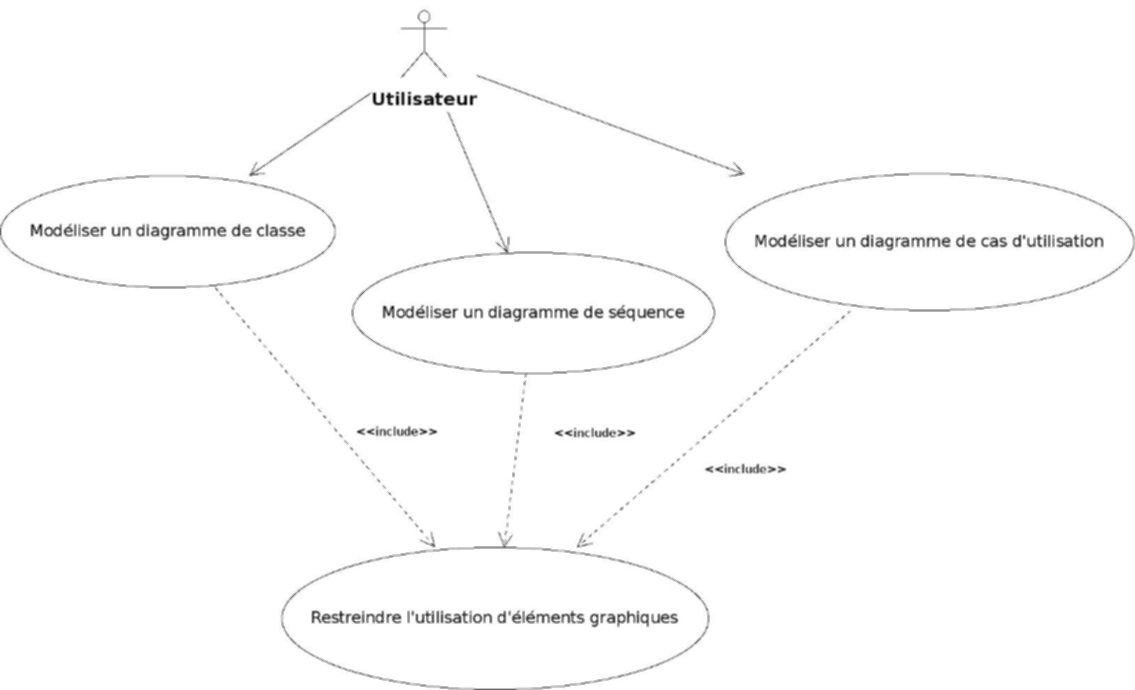
\includegraphics[width=19cm]{casUtilisation.jpg}
		\caption{Diagramme de cas d'utilisation}
	\end{figure}
	\chapter{Conception}
	\section{Architecture générale du projet}
		\vspace{10px}
	\begin{wrapfigure}{l}{7cm}
	\begin{tikzpicture}
		\draw (0,0.0) -- (0,-10.2) ;
		\draw (0.0,-0.0) -- (1.50,-0.0) ;
		\draw (0.0,-10.2) -- (1.50,-10.2) ;
		\node at (1.5,0.2) {\policePackage{eltGraphique}} ;
		\node at (2.0,-0.3) {\textit{ElementGraphique}} ;
		\node at (2.0,-0.7) {\policePackage{eltModelisation}} ;
		\draw (0.3,-1.1) -- (0.3,-7.0) ;
		\draw (0.3,-1.1) -- (0.80,-1.1) ;
		\draw (0.35,-7.0) -- (0.85,-7.0) ;
		\node at (1.27,-1.3) {\textit{Acteur}} ;
		\node at (1.74,-1.7) {ActeurActif} ;
		\node at (1.84,-2.2) {ActeurPassif} ;
		\node at (1.45,-2.7) {Attribut} ;
		\node at (1.99,-3.2) {CasUtilisation} ;
		\node at (1.33,-3.7) {Classe} ;
		\node at (2.6,-4.2) {\textit{ElementModelisation}} ;
		\node at (1.58,-4.7) {Interface} ;
		\node at (1.58,-5.2) {Methode} ;
		\node at (1.75,-5.7) {Traitement} ;
		\node at (1.6,-6.2) {Visibilite} ;
		\node at (1.55,-6.7) {Variable} ;

		\node at (0.9,-7.7) {\policePackage{ligne}} ;
		\draw (0.3,-8.0) -- (0.3,-10.0) ;
		\draw (0.3,-8.0) -- (0.80,-8.0) ;
		\draw (0.3,-10) -- (0.80,-10) ;
		\node at (1.85,-8.3) {Cardinalite} ;
		\node at (1.25,-8.8) {Lien} ;
		\node at (2.57,-9.3) {MessageTraitement} ;
		\node at (1.70,-9.8) {TypeLien} ;
		\node at (1.0,-10.8) {\policePackage{diagramme}} ;

		\draw (0.0,-11.0) -- (0.0,-13.0) ;
		\draw (0.0,-11.0) -- (0.50,-11.0) ;
		\draw (0.0,-13.0) -- (0.50,-13.0) ;
		\node at (1.4,-11.3) {Diagramme} ;
		\node at (2.7,-11.8) {DiagrammeCasUtilisation} ;
		\node at (2.0,-12.3) {DiagrammeClasse} ;
		\node at (2.25,-12.8) {DiagrammeSequence} ;
	\end{tikzpicture}
	\end{wrapfigure}
		L'architecture est la base d'un projet comme le notre, car il sera repris et amélioré par d'autre étudiants. 
		En utilisant la notation UML, nous sommes parvenu à élaborer un ``méta modèle'' de cette notation mais
		en isolant uniquement l'aspect graphique, faisant ainsi abstraction des multiples règles de conception que la norme UML impose.
		Après discussion avec le client, de nombreuses modifications ont été apportées à l'architecture d'origine 
		pour aboutir à une solution stable. Cette nouvelle architecture se compose de vingt classes, réparties 
		en quatre \glo{paquetages.}{Paquetage}{Un paquetage en Java est un regroupement de classes ayant la même thématique.}\\ 

		Dans cet arbre représentant notre architecture, on peut voir certains noms écris en \policePackage{gras}. 
		ou en \textit{italique}. 
		Les noms en \policePackage{gras} représentent les différents paquetages que nous avons séparés.
		
		Ceux en \textit{italiques} sont des classes abstraites crées afin de factoriser le code dans l'optique de réaliser une programmation objet optimale 
		et de suivre les objectifs de propreté du code imposés par le client.\vspace{2px}
	\paragraph{}	
		Dans un premier temps, nous avons séparer les diagrammes des éléments graphiques. En effet, un diagramme sera composé de
		toute sorte d'éléments graphiques. Puis nous avons découper ces derniers en deux, isolant ainsi les lignes des éléments
		de modélisation tels que les classes, les traitements ou les cas d'utilisation.\vspace{2px}
		
		\texttt{ElementGraphique} et \texttt{ElementModelisation} sont des classes abstraites qui regroupent les fonctions communes
		à toutes les classes de leur paquetage respectifs sans pour autant en fournir une implémentation de chacune d'elles -- comme par exemple la méthode qui crée la
		représentation graphique d'un élément ou celle qui permet de le supprimer d'un diagramme.\\ 
	Prenons maintenant chaque paquetage séparément pour vois comment ils fonctionnent plus en détails.
	% Arbre de classe
	\subsection{Paquetage eltGraphique}
	Le paquetage \policePackage{eltGraphique} regroupe toutes les classes qui représentent des éléments graphiques. Il regroupe la classe 
	\textit{ElementGraphique} et deux paquetages \policePackage{eltModelisation} et \policePackage{ligne}. Cette classe possède deux attributs 
	\texttt{graph} et \texttt{diagramme}, correspondant respectivement au graphe dans lequel sont stockés les éléments 
	et le diagramme afficher à l'écran. Elle comprend également (en plus d'un constructeur initialisant les attributs) 
	les méthodes \texttt{supprimer} permettant de supprimer un élément du graphe et du diagramme, ainsi que \texttt{creer}, 
	méthode abstraite réimplémentée dans les classes descendantes servant à créer la représentation graphique de l'objet 
	et de l'afficher sur le diagramme.
	\paragraph{Paquetage eltModelisation} Ce paquetage regroupe toutes les classes représentant les différents éléments de 
	modélisation que l'on trouve dans les diagrammes UML de cas d'utilisation, classe et de séquence. \textit{Acteur} 
	est une classe abstraite car les acteur actifs et passifs ont beaucoup de caractéristiques identiques mais n'ont pas 
	la même représentation sur un diagramme. Les classes \texttt{Visibilite}, \texttt{Methode} et \texttt{Attribut} permettent au client de créer 
	facilement une interface de saisie de ces éléments, facilitant l'usage du logiciel final. De plus, l'ajout de ces 
	méthodes et attributs dans des classes, des acteurs, des traitements ou des interfaces pourra faciliter l'ajout futur 
	de nouvelle fonctionnalités comme par exemple de la génération de code \glo{Java}{Java}{Langage de programmation orienté objet moderne, il compile le programme pour ensuite l'exécuter sur une machine Java, ainsi le programme une fois compilé peut être exécuté sur différentes plateformes (Windows, Linux, Mac OS X, \ldots).}.
	\paragraph{Paquetage ligne} Ce paquetage regroupe peu de classe. \texttt{TypeLien} est une classe énumérée servant à recenser
	tous les types graphiques de liens existant dans la notation UML. \texttt{Cardinalite} quant à elle, permet comme \texttt{Methode} 
	ou \texttt{Attribut}, d'aider le client à permettre un saisie facilité des cardinalités d'un lien dans un diagramme de classe par exemple.
	La classe \texttt{Lien} comprend la méthode \texttt{creer} qui va configurer tous les styles de liens et appliquer au nouveau lien
	le style choisi par l'utilisateur. \texttt{MessageTraitement} spécialise Lien, permettant de créer un style de lien particulier
	aux messages entre traitement dans les diagrammes de séquences.
	\subsection{Paquetage diagramme}
	La paquetage \policePackage{diagramme} comprend plusieurs type de diagramme prédéfinis qui sont cas d'utilisation, classe et séquence.
	Ils descendent de la classe \texttt{Diagramme}. Chaque type de diagramme implémente deux méthode \texttt{eltAutorise} et \texttt{lienAutorise}
	qui permettent respectivement d'autoriser ou interdire un type d'élément particulier et un type de lien entre deux types d'éléments
	particuliers. La classe Diagramme est générique. Par défaut elle autorise tous les éléments et tous les liens. Il est donc possible
	au client de réimplémenter ses propres méthodes pour créer ses propres règles.

	\section{Conception détaillée}
	\subsection{Documentation}
	La description détaillée des méthodes et des attributs de chaque classe est disponible sous forme numérique
	avec la recette ainsi qu'en trois exemplaires différents aux adresses suivantes \\
	$\rhd$ \url{http://documentation.joohoo.fr/libUML/public} (Documentation publique et protégée)\\
	$\rhd$ \url{http://documentation.joohoo.fr/libUML/private} (Documentation publique, protégées et pri\-vée)\\
	$\rhd$ \url{http://documentation.joohoo.fr/libUML/junitTests} (Tests unitaires)\\	
	\subsection{Relations entre les classes}	
	Le diagramme de paquetage est disponible à l'annexe \ref{diagrammePaquetage} page \pageref{diagrammePaquetage}. Celui-ci vous permettra de repérer les 
	relations entre les classes.
	
	\appendix
	\closeout\glossaireVar
	\chapter{Glossaire}\label{glossaire}
	\begin{sortedlist}
		\chapter {Glossaire}

	\end{sortedlist}
	\chapter{Diagramme de paquetage} \label{diagrammePaquetage}
	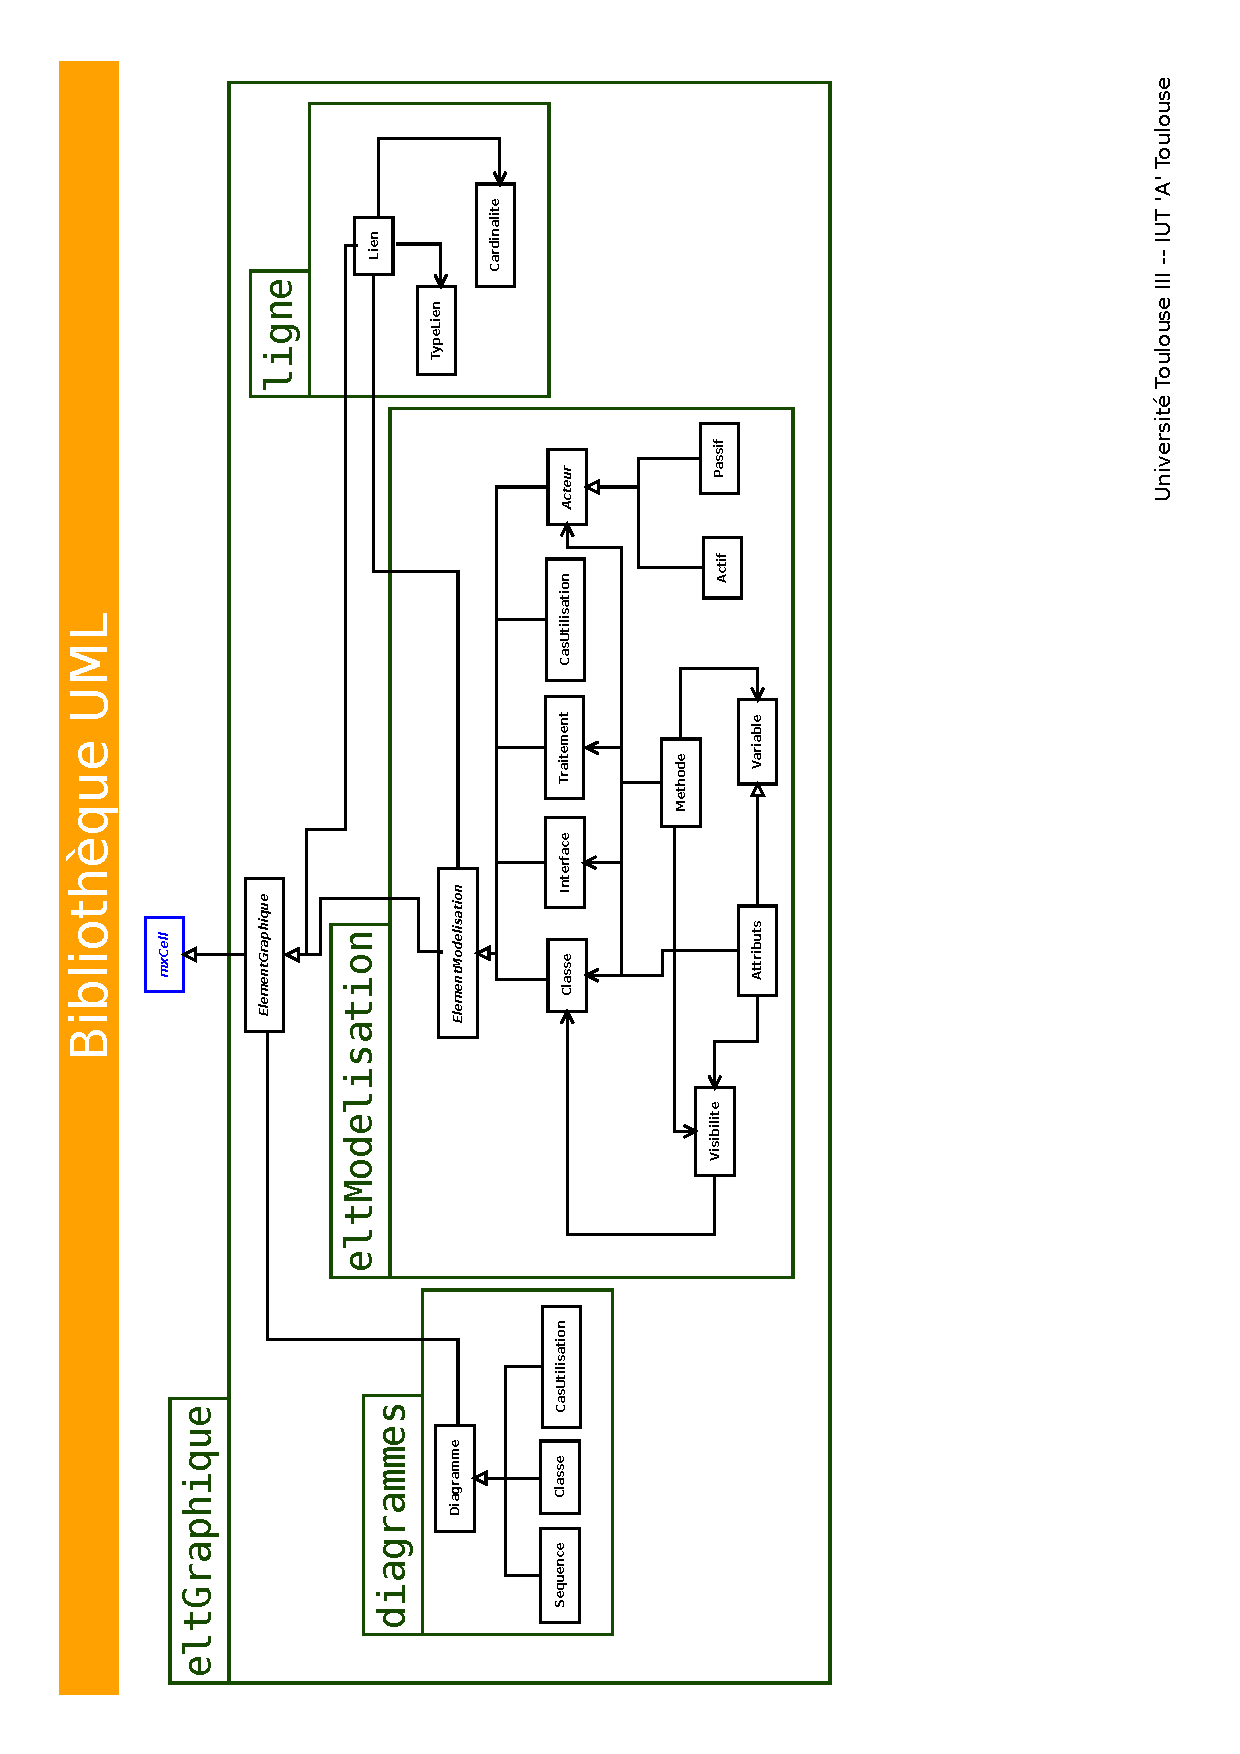
\includepdf[page=1]{paquetageSansMethodes.pdf}
\end{document}
